\documentclass[notheorems, aspectratio=169, 12pt, unicode]{beamer}
\usepackage{mysettings}
\begin{document}

\begin{frame}
 \titlepage
\end{frame}

 \section{Introduction}
 
 \begin{frame}<handout:0>{自己紹介}
  \begin{itemize}
   \item PN : そくらてす
   \item 普段やっていること : \pause
	 \begin{itemize}
	  \item 某大学計算機科学系の学科の博士課程の学生
		\begin{itemize}
		 \item \alert{計算機科学何もわからん(ノдヽ)} \pause
		 \item \alert{数学何もわからん(ノдヽ)} \pause
		 \item \alert{任意の概念何もわからん(ノдヽ)} \pause
		 \item けんきゅーしてること : 証明論のようなもの \pause
		\end{itemize}
	  \item \structure{Twitter} でくだを巻く \pause 
	 \end{itemize}
   \item 間違ったこと言ったら教えてね
  \end{itemize} 
 \end{frame}
 
 \section{Separation Logic}

 \begin{frame}{分離論理とは?}
  \begin{itemize}
   \item \alert{分離論理}とは? \pause
	 \begin{itemize}
	  \item \alert{ヒープ領域}に言及できる論理体系
	  \item \alert{ヒープ領域}の状態を表す記法 \pause
	 \end{itemize}
   \item \alert{ヒープ領域}とは? \pause
	 \begin{itemize}
	  \item C言語などの\alert{ポインタ}で触ることのできるメモリの領域 \pause
		(と思っといてくれ) 
	 \end{itemize}
  \end{itemize} 
 \end{frame}

 \begin{frame}{分離論理の論理式}
 \begin{definition}[分離論理の論理式]
  \minusbaselineskip
  \begin{align*}
   &\text{Variables(変数記号)}  &x &\in \mathVar \\
   &\text{Terms(項)}  &t &::= \mathvalnil \mathrelbar x \\
   &\text{Atomic Formul\ae(原子論理式)}  &\alpha &::= \mathemp \mathrelbar  t = t  \mathrelbar \alert{\mathpointer{t}{1}{t}} \mathrelbar  \alert{\mathpointer{t}{2}{t{,}\ t}} \mathrelbar \\
   & & &\phantom{{}::={}}  \alert{\mathprls{t}{t}} \mathrelbar \alert{\mathprtree{t}}  \\
   &\text{Formul\ae(論理式)}  &\varphi &::= \alpha \mathrelbar \lnot \varphi \mathrelbar \varphi \land \varphi \mathrelbar \exists x.\varphi \mathrelbar \alert{\varphi \mathsepstar \varphi} \mathrelbar \alert{\varphi \mathmagicwand \varphi} \\
  \end{align*}
 \end{definition}
 \end{frame}

 \begin{frame}{分離論理の意味のイメージ}{$\mapsto$}
  \begin{table}[tbh]
   \begin{tabular}{cc}
    \begin{minipage}{0.3\hsize}
     \begin{center}
      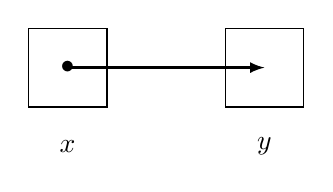
\begin{tikzpicture}
       \draw (0,0) rectangle +(1,1);
       \draw (2.5,0) rectangle +(1,1);
       \draw (0.5,0.5) node{$\bullet$};
       \draw[-latex,thick] (0.5,0.5) -- (3.0,0.5); 
       \draw (0.5,-0.5) node{$x$};
       \draw (3.0,-0.5) node{$y$};
      \end{tikzpicture}
     \end{center}     
    \end{minipage}
     &
     \begin{minipage}{0.3\hsize}
      \begin{center}
       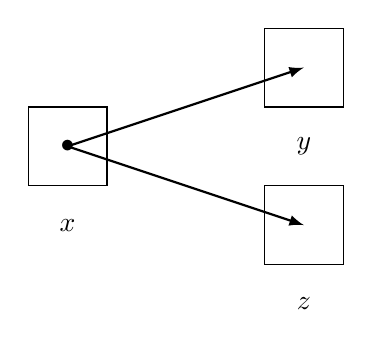
\begin{tikzpicture}
        \draw (-0.5,-0.5) rectangle +(1,1);
        \draw (2.5,0.5) rectangle +(1,1);
        \draw (2.5,-1.5) rectangle +(1,1);

	\draw (0.0,0.0) node{$\bullet$};
	\draw[-latex,thick] (0.0,0.0) -- (3.0,1.0);
	\draw[-latex,thick] (0.0,0.0) -- (3.0,-1.0);

        \draw (0.0,-1.0) node{$x$};
        \draw (3.0,-0.0) node{$y$};
        \draw (3.0,-2.0) node{$z$};
       \end{tikzpicture}
      \end{center}
     \end{minipage} \\
     $\mathpointer{x}{1}{y}$ & $\mathpointer{x}{2}{y{,}\ z}$
   \end{tabular}
  \end{table} 
 \end{frame}

\begin{frame}{分離論理の意味のイメージ}{$\mathsepstar$}
  \begin{table}[tbh]
    \begin{tabular}{ccc}
     \begin{minipage}{0.3\hsize}
     \begin{center}
      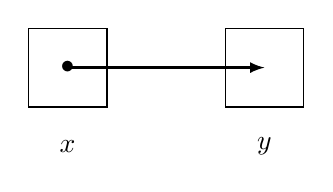
\begin{tikzpicture}
       \draw (0,0) rectangle +(1,1);
       \draw (2.5,0) rectangle +(1,1);
       \draw (0.5,0.5) node{$\bullet$};
       \draw[-latex,thick] (0.5,0.5) -- (3.0,0.5); 
       \draw (0.5,-0.5) node{$x$};
       \draw (3.0,-0.5) node{$y$};
      \end{tikzpicture}
     \end{center}     
    \end{minipage}
     &\begin{minipage}{0.05\hsize}
       \begin{center}
	\begin{tikzpicture}
	 \draw (0,0) node{$\mathsepstar$};
	 \draw (0,-0.5) node{\phantom{$x$}};
	\end{tikzpicture}
       \end{center}     
      \end{minipage}
	 &\begin{minipage}{0.3\hsize}
	   \begin{center}
	    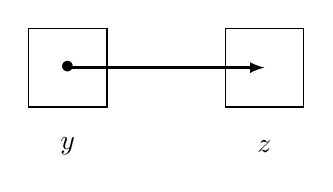
\begin{tikzpicture}
	     \draw (0,0) rectangle +(1,1);
	     \draw (2.5,0) rectangle +(1,1);
	     \draw (0.5,0.5) node{$\bullet$};
	     \draw[-latex,thick] (0.5,0.5) -- (3.0,0.5); 
	     \draw (0.5,-0.5) node{$y$};
	     \draw (3.0,-0.5) node{$z$};
	    \end{tikzpicture}
	   \end{center}     
	  \end{minipage} \\
     $\mathpointer{x}{1}{y}$ & $\mathsepstar$ & $\mathpointer{y}{1}{z}$
    \end{tabular}
  \end{table}
 \begin{center}
  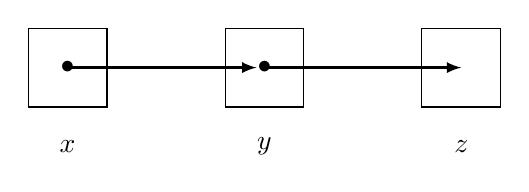
\begin{tikzpicture}
   \draw (0,0) rectangle +(1,1);
   \draw (2.5,0) rectangle +(1,1);
   \draw (5.0,0) rectangle +(1,1);
   
   \draw (0.5,-0.5) node{$x$};
   \draw (3.0,-0.5) node{$y$};
   \draw (5.5,-0.5) node{$z$};
   
   \draw (0.5,0.5) node{$\bullet$};
   \draw[-latex,thick] (0.5,0.5) -- (2.9,0.5);
   \draw (3.0,0.5) node{$\bullet$};
   \draw[-latex,thick] (3.0,0.5) -- (5.5,0.5);
  \end{tikzpicture} \\
  $\mathpointer{x}{1}{y}\mathsepstar \mathpointer{y}{1}{z}$
 \end{center}
\end{frame}

\begin{frame}{分離論理の意味のイメージ}{$\mathprls{\mathdash}{\mathdash}$}
 \begin{center}
  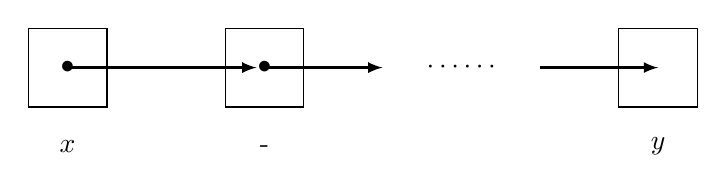
\begin{tikzpicture}
   \draw (0,0) rectangle +(1,1);
   \draw (0.5,-0.5) node{$x$};
   \draw (0.5,0.5) node{$\bullet$};

   \draw (2.5,0) rectangle +(1,1);
   \draw (3.0,-0.5) node{-};
   \draw (3.0,0.5) node{$\bullet$};

   \draw (5.5,0.5) node{$\cdots\cdots$};

   \draw (7.5,0) rectangle +(1,1);
   \draw (8.0,-0.5) node{$y$};
   
   \draw[-latex,thick] (0.5,0.5) -- (2.9,0.5);
   \draw[-latex,thick] (3.0,0.5) -- (4.5,0.5);
   \draw[-latex,thick] (6.5,0.5) -- (8.0,0.5);
  \end{tikzpicture} \\
  $\mathprls{x}{y}$
 \end{center}
\end{frame}

\begin{frame}{分離論理の意味のイメージ}{$\mathprtree{\mathdash}$}
\begin{center}
 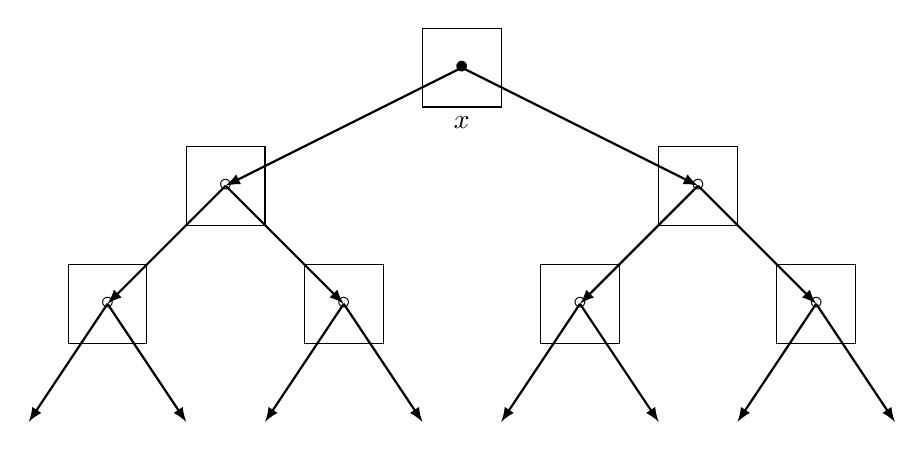
\begin{tikzpicture}
  \draw (0,0) node{$\bullet$};
  \draw (-0.5,-0.5) rectangle +(1,1);
  \draw (0,-0.7) node{$x$};

  \draw (-3.0,-1.5) node{$\circ$};
  \draw (-3.5,-2.0) rectangle +(1,1);

  \draw (3.0,-1.5) node{$\circ$};
  \draw (2.5,-2.0) rectangle +(1,1);

  \draw (-4.5,-3.0) node{$\circ$};
  \draw (-5.0,-3.5) rectangle +(1,1);

  \draw (-1.5,-3.0) node{$\circ$};
  \draw (-2.0,-3.5) rectangle +(1,1);

  \draw (1.5,-3.0) node{$\circ$};
  \draw (1.0,-3.5) rectangle +(1,1);

  \draw (4.5,-3.0) node{$\circ$};
  \draw (4.0,-3.5) rectangle +(1,1);

  \draw[-latex,thick] (0.0,0.0) -- (3.0,-1.5);
  \draw[-latex,thick] (0.0,0.0) -- (-3.0,-1.5);

  \draw[-latex,thick] (3.0,-1.5) -- (4.5,-3.0);
  \draw[-latex,thick] (3.0,-1.5) -- (1.5,-3.0);

  \draw[-latex,thick] (-3.0,-1.5) -- (-4.5,-3.0);
  \draw[-latex,thick] (-3.0,-1.5) -- (-1.5,-3.0);

  \draw[-latex,thick] (4.5,-3.0) -- (5.5,-4.5);
  \draw[-latex,thick] (4.5,-3.0) -- (3.5,-4.5);

  \draw[-latex,thick] (1.5,-3.0) -- (2.5,-4.5);
  \draw[-latex,thick] (1.5,-3.0) -- (0.5,-4.5);

  \draw[-latex,thick] (-4.5,-3.0) -- (-5.5,-4.5);
  \draw[-latex,thick] (-4.5,-3.0) -- (-3.5,-4.5);

  \draw[-latex,thick] (-1.5,-3.0) -- (-2.5,-4.5);
  \draw[-latex,thick] (-1.5,-3.0) -- (-0.5,-4.5);
 \end{tikzpicture} \\
 $\mathprtree{x}$
\end{center}
\end{frame}

\section{Program verification}

\begin{frame}{プログラム検証とは?}
 \begin{itemize}
  \item \alert{プログラム検証}とは? \pause
	\begin{itemize}
	 \item プログラムが持っていてほしい性質を持っているか
	 どうかを数学的に保証すること \pause
	\end{itemize}
  \item プログラムが持っていてほしい性質とは? \pause
	\begin{itemize}
	 \item 仕様を満たしているか?
	       (\alert{部分正当性})
	 \item プログラムはきちんと停止するか?
	       (\alert{停止性})
	 \item エラーを吐かないか?
	       (\alert{安全性})
	       \quad etc.
	\end{itemize}
 \end{itemize}
\end{frame}

\begin{frame}<handout:0>{プログラム検証の例のようなもの}\setstretch{1}
 \minusbaselineskip
 \begin{align*} 
  & \mathprogramsy{deltree(*x)} \{  \\
  &\quad \mathprogramsy{if\left(x=NULL\right)\ return\ 0;} \\
  &\quad  \mathprogramsy{else \{} \\
  &\qquad \mathprogramsy{l := x.left;} \\ 
  &\qquad \mathprogramsy{r := x.right;} \\
  &\qquad  \mathprogramsy{deltree(l);} \\ 
  &\qquad \mathprogramsy{deltree(r);}  \\
  &\qquad  \mathprogramsy{free(x);} \\
  &\quad \mathprogramsy{\}} \\
  &\mathprogramsy{\}}
 \end{align*} 
\end{frame}

\begin{frame}<handout:0>{プログラム検証の例のようなもの}
 \begin{center}
  \begin{tikzpicture}
   \onslide+<1-3>{ \draw (0,0) node{$\bullet$};
   \draw (-0.5,-0.5) rectangle +(1,1);
  \draw (0,-0.7) node{$\mathprogramsy{x}$};}

   \onslide+<1>{ \draw[-latex,thick] (0.0,0.0) -- (-3.0,-1.5);
   \draw (-3.3,-1.75) node{$\mathprtree{\mathprogramsy{l}}$};}

   \onslide+<1-2>{\draw[-latex,thick] (0.0,0.0) -- (3.0,-1.5);
  \draw (3.3,-1.75) node{$\mathprtree{\mathprogramsy{r}}$};
}
  \end{tikzpicture}\\
  \onslide<4>{\alert{DELETE TREE !!!}}
 \end{center}
\end{frame}

\begin{frame}{プログラム検証の例のようなもの}
 \setstretch{0.1}
 \minusbaselineskip
 \minusbaselineskip
 \begin{align*}
  & \alert{\left\{\mathprtree{\mathprogramsy{x}}\right\}} \\
  & \mathprogramsy{deltree(*x)} \{  \\
  &\quad \mathprogramsy{if\left(x=NULL\right)\ return\ 0;} \quad \onslide+<2->{\alert{\left\{\mathemp\right\}}} \\
  &\quad  \mathprogramsy{else \{} \quad \onslide+<3->{\alert{\left\{\mathpointer{\mathprogramsy{x}}{2}{y{,}\ z} \mathsepstar \mathprtree{y} \mathsepstar \mathprtree{z}\right\}}} \\
  &\qquad \mathprogramsy{l := x.left;} \quad \onslide*<4|handout:0>{\alert{\left\{\mathprogramsy{l}=y \land \mathpointer{\mathprogramsy{x}}{2}{y{,}\ z} \mathsepstar \mathprtree{y} \mathsepstar \mathprtree{z}\right\}}}
\onslide*<5|handout:0>{\alert{\left\{\mathpointer{\mathprogramsy{x}}{2}{\mathprogramsy{l}{,}\ z} \mathsepstar \mathprtree{\mathprogramsy{l}} \mathsepstar \mathprtree{z} \right\}}} \ \mathprogramsy{r := x.right;} \quad \onslide*<6|handout:0>{\alert{\left\{\mathprogramsy{r}=z \land \mathpointer{\mathprogramsy{x}}{2}{\mathprogramsy{l}{,}\ z} \mathsepstar \mathprtree{\mathprogramsy{l}} \mathsepstar \mathprtree{z}\right\}}} \onslide*<7->{\alert{\left\{\mathpointer{\mathprogramsy{x}}{2}{\mathprogramsy{l}{,}\ \mathprogramsy{r}} \mathsepstar \mathprtree{\mathprogramsy{l}} \mathsepstar \mathprtree{\mathprogramsy{r}}\right\}}}\\
  &\qquad  \mathprogramsy{deltree(l);} \quad \onslide*<8->{\alert{\left\{\mathpointer{\mathprogramsy{x}}{2}{\mathprogramsy{l}{,}\ \mathprogramsy{r}} \mathsepstar \mathemp \mathsepstar \mathprtree{\mathprogramsy{r}}\right\}}}\\ 
  &\qquad \mathprogramsy{deltree(r);} \quad \onslide*<9->{\alert{\left\{\mathpointer{\mathprogramsy{x}}{2}{\mathprogramsy{l}{,}\ \mathprogramsy{r}} \mathsepstar \mathemp\right\}}} \\
  &\qquad  \mathprogramsy{free(x);} \quad \onslide*<10->{\alert{\left\{ \mathemp\right\}}}\\
  &\quad \mathprogramsy{\}} \quad \onslide*<11->{\alert{\left\{ \mathemp\right\}}} \\
  &\mathprogramsy{\}} \quad \alert{\left\{\mathemp\right\}}
 \end{align*} 
\end{frame}

\section{References}

\begin{frame}{参考文献}
 \begin{thebibliography}{9}
  \bibitem{Reynolds2002} John C. Reynolds, ``Separation Logic: A Logic for Shared Mutable Data Structure'', Proceedings of the 17th Anual IEEE Symposium on Logic in Computer Science, 2002.
  \bibitem{Brotherston2015} James Brotherston, 
	  `` An introduction to separation logic '', 
	  Logic Summer School, ANU, 7 December 2015.
\bibitem{Sokratesnil2020} Sokratesnil,『分離論理入門のようなもの』,\url{}
 \end{thebibliography} 
\end{frame}

\appendix

 \begin{frame}{分離論理の意味}{$\mathmagicwand$}
  \[
  \varphi * \psi \vdash \vartheta \iff \varphi \vdash \psi \mathmagicwand \vartheta
  \]
  
 \begin{ex}
  \[
  \mathprls{x}{y} * \mathprls{y}{z} \vdash \mathprls{x}{z} \iff \mathprls{x}{y} \vdash \mathprls{y}{z} \mathmagicwand \mathprls{x}{z}
  \]
 \end{ex}
 \end{frame}
 
 \begin{frame}{Frame Rule}
  \begin{definition}[Frame rule]
   \begin{prooftree}
    \AxiomC{$\left\{P\right\} C \left\{Q\right\}$}
    \UnaryInfC{$\left\{P \mathsepstar R\right\} C \left\{Q \mathsepstar R\right\}$}
   \end{prooftree}
  \end{definition}
  \begin{rem}
   一般に次は成立しない。
   \begin{prooftree}
    \AxiomC{$\left\{P\right\} C \left\{Q\right\}$}
    \UnaryInfC{$\left\{P \land R\right\} C \left\{Q \land R\right\}$}
   \end{prooftree}
  \end{rem}
 \end{frame}

 \begin{frame}{Symbolic heap}
  \begin{definition}[Symbolic heap]
  \minusbaselineskip
  \begin{align*}
   &\text{Variables}  &x &\in \mathVar \\
   &\text{Terms}  &t &::= \mathvalnil \mathrelbar x \\
   &\text{Pure Formul\ae}  &\Pi &::=   t = t  \mathrelbar t \neq t \mathrelbar \top \mathrelbar \bot \mathrelbar \Pi \land \Pi \\
   &\text{Spatial Formul\ae}  &\Sigma &::= \mathemp \mathrelbar \mathpointer{t}{1}{t} \mathrelbar  \mathpointer{t}{2}{t{,}\ t} \mathrelbar  \mathprls{t}{t} \mathrelbar \mathprtree{t} \mathrelbar \Sigma \mathsepstar \Sigma \\
   &\text{Formul\ae}  &\varphi &::=  \Pi \land \Sigma
  \end{align*}
 \end{definition}
 \end{frame}

\end{document}
